\documentclass{llncs}
\usepackage[utf8]{inputenc}
\usepackage{todonotes}
\usepackage{amsmath}
\usepackage{textcomp} % for \textdegree
\usepackage[hidelinks]{hyperref}
\usepackage{cleveref}
\usepackage{xstring}
\usepackage{booktabs}
\usepackage{tikz}
\usetikzlibrary{arrows,snakes,patterns,matrix,shapes,fit,calc,shadows,plotmarks,decorations.pathmorphing,decorations.markings,backgrounds}
\usetikzlibrary{external}
\tikzexternalize
\tikzsetexternalprefix{fig/}

\usepackage{pgfplots}
\pgfplotsset{compat=1.4, width=0.9\columnwidth, height=0.6\columnwidth}

\newcommand{\inputtikz}[1]
{
  \StrSubstitute{#1}{/}{.}[\fn]
  \scancs{\filename}{\fn}
  \tikzsetfigurename{\filename}
  \input{#1.tikz}
}

\graphicspath{{fig/}}
%%%%%%%%%%%%%%%%%%%%%%%%%%%%%%%%%%%%%%%%%%%%%%%%%%%%%%%%%%%%%%%%%%%%%%%%%%%%%%%%
\begin{document}

\title{SimSpark: An Open Source Robot Simulator Developed by RoboCup Community}

\author{Yuan Xu\inst{1} \and Hedayat Vatankhah\inst{2}}

\institute{
\begin{minipage}[t]{0.4\textwidth}
\centering
DAI-Labor \\
Technische Universität Berlin \\
Ernst-Reuter-Platz 7, Berlin \\
D-10587 Germany\\
\email{yuan.xu@dai-labor.de}
\end{minipage}
\begin{minipage}[t]{0.4\textwidth}
\and
\centering
Amirkabir University of Technology, Iran\\
\email{hedayatv@gmail.com}
\end{minipage}
}

\maketitle

\begin{abstract}
  this is abstract
\end{abstract}

\section{Introduction}

\todo[inline]{Background/histsory}
\cite{Boedecker2008,OR05}

\todo[inline]{Releated work: SimRobot, Webots, V-REP, Gazebo...}

\section{Current state / development since 2008}
Because last paper about simspark was in 2008
\todo[inline]{sensors: ACC, FSR, restict vision, with line perceptions, image ...}
\todo[inline]{robot model: NAO}
\todo[inline]{soccer rules (referee)}
\todo[inline]{bigger fields and more robots}

\section{Recent Development (Changes 2013)}


\subsection{realistic motor modelling}
NAO robot has twenty-one motor joints as its actuators.
The simple motor model is one reason for the unrealistic simulation results.
The ODE provides a simple model of real life servos.
It has two parameters: a desired speed and the maximum force that is available to reach that speed. The motor brings the body up to speed in one step; and provides force that is not more than is allowed.
There is no motor that works like this in reality.
Furthermore, some aspects like stiffness control, power consumption and temperature regulation, are missing but are also important for robotics.


A PD controller was implemented for the simulated NAO. \todo{this is for angle position control like DCM of NAO}

\paragraph{Stiffness}
The stiffness determines how strong the motor is. The value is from 0.0
to 1.0, 0 means the motor is off and 1 means the motor is running at
full power. In the real robot,
this percentage is the maximum electric current applied to the motor. Setting the
stiffness to 0.5 means that the electric current limitation is reduced
to 50\%.

For a DC motor, the electric current, $I$, determines the output torque,
$\tau$:
\begin{align}
  \tau &= K_\tau I \label{eq:tau-i}
\end{align}
where $K_\tau$ is the torque constant of the motor. It can be found in the
specifications from \cite{naoqi}. In
the simulation, the maximum torque of the servo can be specified, therefore the
stiffness control can be easily implemented by setting the maximum torque
of the simulated servo:
\begin{align}
  \tau_{max}(t) &= k_{s}(t) T_{max}
\end{align}
where $\tau_{max}(t)$ is the maximum torque set in the simulated servo at
time $t$; $k_{s}(t)$ is the stiffness at time $t$; and $T_{max}$
denotes the maximum torque of the servo when stiffness is 1.

\paragraph{Power Consumption}
Another important aspect besides the motor's performance is its
power consumption: how much energy does it cost to run.
The robot is powered by a battery with limited energy, and has to walk during the
game: half a game is 10 minutes.
An even more important factor in energy consumption is
that the motor can overheat if it consumes too much energy and
becomes too hot. In the real NAO, Aldebaran Robotics estimates the temperature
of each motor by integrating electric current, and shuts down the motor
when the temperature is too high. Therefore modeling power consuming
is important for implementing energy effective motions.

DC motors are based on the following equations:
\begin{align}
  U &= U_e + IR \label{eq:u-ir}\\
  U_e &= K_e \dot{\theta} \label{eq:u-ke}
\end{align}
where $U$ is the voltage of input, $U_e$ is the back electromotive
force (EMF), $I$ is the electric current, $R$ is resistance,
$\dot{\theta}$ is the speed, and $K_e$ is the speed constant of the motor.

The value of $R$ and $K_e$ can be found in the specifications from \cite{naoqi};
and the simulation engine provides
the value of $\tau$ and $\dot{\theta}$; therefore we can calculate the
power consumption by putting \cref{eq:tau-i,eq:u-ir,eq:u-ke} together:
\begin{align}
  P &= UI \\
  &= U_eI + I^2R \\
  &= \frac{K_e}{K_\tau}\dot{\theta}\tau + \frac{R}{K_\tau^2}\tau^2
\end{align}

And the total energy used by the motor is:
\begin{equation}
  \label{eq:motor-power}
  E = \sum_t{P_t\Delta{}t}
\end{equation}
where $\Delta{}t$ is the time step of the simulation, and $P_t$ is the power consumed at time $t$. 

\Cref{fig:battery} compares the simulation result of this model to
reality. In this example, the robot turns left for 5 minutes, then
stands for 1 minutes and then turns right for 5 minutes. This is shown by the change of electric current in the figure. For the overall
power consumption, the energy consumed by devices other than motors,
e.g. mainboard, CPU, camera, etc. has to be added. It is the power
consumption of the robot in an idle state (all motors are off), and measured to be 33 W.
\begin{figure}
  \centering
  \inputtikz{battery}
  \caption{Power consumption of the real and the simulated robot in action.
    The electric current is the summary of all motors.}
  \label{fig:battery}
\end{figure}

\paragraph{Temperature Regulation}
We model the temperature and heat of the motor with the following equations:
\begin{align}
  \Delta{}Q^+ &= I^2R\Delta{}t \\
  \Delta{}Q^- &= -\lambda(T-T_e)\Delta{}t \\
  \Delta{}Q &= \Delta{}Q^+ + \Delta{}Q^-\\
  C &= \frac{\Delta{}Q}{\Delta{}T}
\end{align}
where $T$ is the temperature of the motor, $T_e$
is the temperature of the environment, but it is the internal temperature
of motor, so it is higher than outside and differs from motor to
motor, $\Delta{}Q^+$ is the heat produced by the motor, $\Delta{}Q^-$ is
the heat transferred from the motor to the environment, $\Delta{}Q$ is the
heat changing, $\lambda$ is thermal conductivity which indicates the
ability of a motor to conduct heat, and $C$ is the heat capacity of
the motor, which can be seen as constant. Finally, the temperature of
the motor at time $t+\Delta{}t$ can be solved as:
\begin{equation}
  \label{eq:motor-temp}
  T_{t+\Delta{}t} = T_t + \Delta{}T = T_t + \frac{[I^2R-\lambda(T_t-T_e)]\Delta{}t}{C}
\end{equation}

In this model, we determined $T_e$, $\lambda$, and $C$ by experiments. It can be formulate as a classic linear regression problem. We rewrite \cref{eq:motor-temp} to:
\begin{align}
  \label{eq:motor-temp-ols}
  \Delta{}tx_0 + T_t\Delta{}tx_1 - \Delta{}t x_2 &= I^2R \\
  x_0 &= C \\
  x_1 &= \lambda \\
  x_2 &= \lambda Te
\end{align}
A sequence values of $\Delta{}t$, $T_t$, and $I^2R$ can be measured by experiment, therefore the optimum values for $x_0$, $x_1$, and $x_2$ can be obtained by linear least squares method, so the parameters of \cref{eq:motor-temp} is determined. \Cref{tab:motor-parameter} gives the results of the experiment.
\begin{table}[h]
  \centering
  \caption{Parameters $T_e$, $\lambda$ and $C$ in the \cref{eq:motor-temp} for different joints of the NAO V3.}
  \label{tab:motor-parameter}
  \begin{tabular}{lccc}
    \toprule
    Joints      & $T_e$ (\textdegree{}C) & $\lambda$ (W/\textdegree{}C) & $C$ (J/\textdegree{}C)\\
    \midrule
    HipYawPitch & 33 & 0.0158 & 27.2 \\
    \midrule
    HipRoll     & & & \\
    AnkleRoll   & 27 & 0.0158 & 27.2 \\
    \midrule
    HipPitch    & & & \\
    KneePitch   & 27 & 0.0198 & 43.6 \\
    AnklePitch  & & & \\
    \bottomrule
  \end{tabular}
\end{table}

After determining the parameters in the \cref{eq:motor-temp}, we can use this model to simulate motor temperature. In \Cref{fig:joint-temperature}, the simulated temperature is compared with data from the real robot.
\begin{figure}
  \centering
  \pgfplotsset{width=0.88\columnwidth}
  \inputtikz{joint-temp-LKneePitch}
  \caption{The temperature of the (knee pitch) motor in the simulation and the real robot. The green background is the electric current in the real robot. The result shows the simulated temperature is very close to the values of the real robot.}
  \label{fig:joint-temperature}
\end{figure}

The whole process of joint simulation is summarized in
\Cref{fig:joint}: stiffness is simulated by setting the maximum torque of
the motor; desired speed of motor is determined by a PD controller
according to the target angle (see \cref{eva-joint-motor}), current angle and current speed; backlash\todo{update: no backlash and PD controller, add feed back of temperature and battery limits}
is modeled by the dead band model; and the simulation engine computes
the resulted angle and torque applied; in the end, the consumed power
and temperature are computed by \cref{eq:motor-power,eq:motor-temp}
respectively.
\begin{figure}
  \centering
  \inputtikz{joint}
  \caption{Pipeline of the servo motor simulation}
  \label{fig:joint}
\end{figure}

\subsection{Heterogeneous Robots}

\subsection{Agent Proxies}

\subsection{Player Integration??}

\section{Applications}

\paragraph{RoboCup simulation league (of course)}

\paragraph{research (used by teams have real robot)}
- we (NaoTH) have shared common interface with NAO
- FUmanoid
- education

\begin{figure}
  \centering
  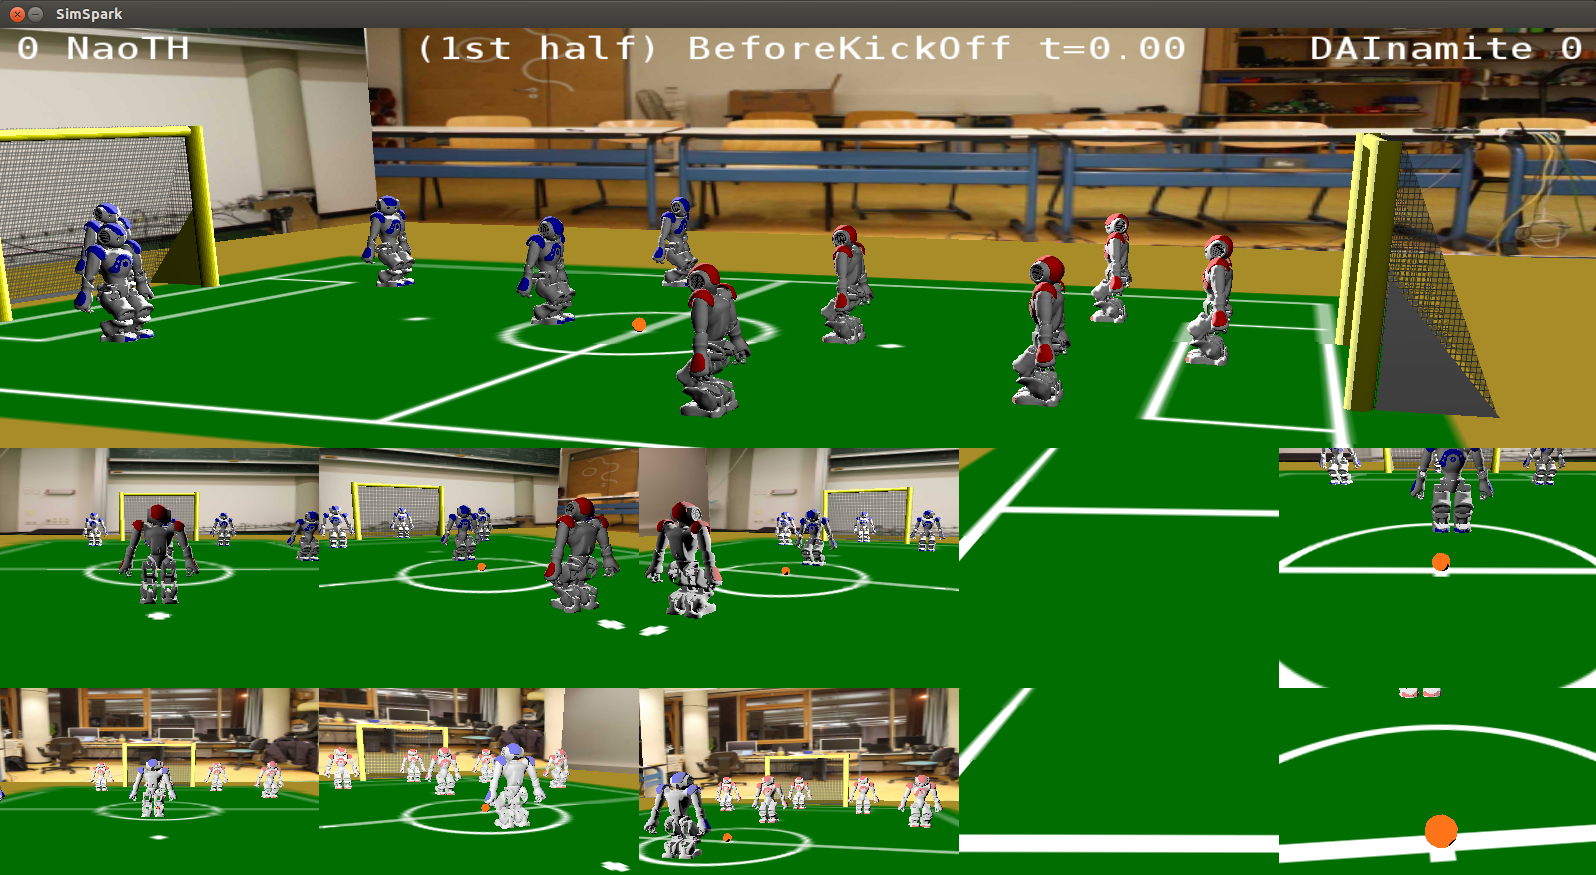
\includegraphics[width = 0.95\columnwidth]{simspark-spl}
  \caption{Prototype of the extended SimSpark for Standard Platform League.
    It simulates a game in our lab. The bottom of screen are images of robot cameras.}
  \label{f:nao-models}
\end{figure}

\section{Conclusion and Future Work}

\bibliographystyle{splncs03}
\bibliography{reference}
\end{document}
